\begin{tehtavasivu}

% tässä ei käytetä konsistenssin vuoksi euromerkkiä \euro (textmode), vaan sanallista ilmaisua ''euro''

% FIXME: Tee vielä toinen tehtävä perusarvosta ``Kirjan myyntihinta'' -tehtävän lisäksi

% FIXME: laaja tehtävä ansio- ja pääomatulojen verotuksesta

\begin{tehtava}
    Laske
    \begin{alakohdat}
	  \alakohta{$4{,}5\,\%$ luvusta 1500}
	  \alakohta{$4{,}5\,\%$ luvusta $b$}
	  \alakohta{$15{,}3\,\%$ luvusta $b$}
	  \alakohta{$152\,\%$ luvusta $b$}
	  \alakohta{$3550\,\%$ luvusta $b$}
    \end{alakohdat}
    \begin{vastaus}
	  \begin{alakohdat}
		\alakohta{67,5}
		\alakohta{$0{,}045b$}
		\alakohta{$0{,}153b$}
		\alakohta{$1{,}52b$}
		\alakohta{$35{,}5b$}
	  \end{alakohdat}
    \end{vastaus}
\end{tehtava}

\begin{tehtava}
    Kuinka monta prosenttia
    \begin{alakohdat}
	  \alakohta{15 on luvusta 75}
	  \alakohta{120 on luvusta 80}
	  \alakohta{400 on luvusta 3,5}
	  \alakohta{luku 50 on lukua 170 pienempi}
	  \alakohta{luku 170 on lukua 50 suurempi}
	  \alakohta{400 on lukua 3,5 suurempi}
    \end{alakohdat}
    \begin{vastaus}
	  \begin{alakohdat}
		\alakohta{\item 20 \%}
		\alakohta{150 \%}
		\alakohta{11428,6 \%}
		\alakohta{70,6 \%}
		\alakohta{240 \%}
		\alakohta{11328,6 \%}
	  \end{alakohdat}
    \end{vastaus}
\end{tehtava}

\begin{tehtava}
    Oppikirjamaraton-tiimi kävi lounastamassa. Osoita oheisen kuitin tiedoilla vääräksi yleinen virhekäsitys,
    että $13\,\%$ suuruisen arvonlisäveron osuus olisi $13\,\%$ lopullisesta myyntihinnasta.
    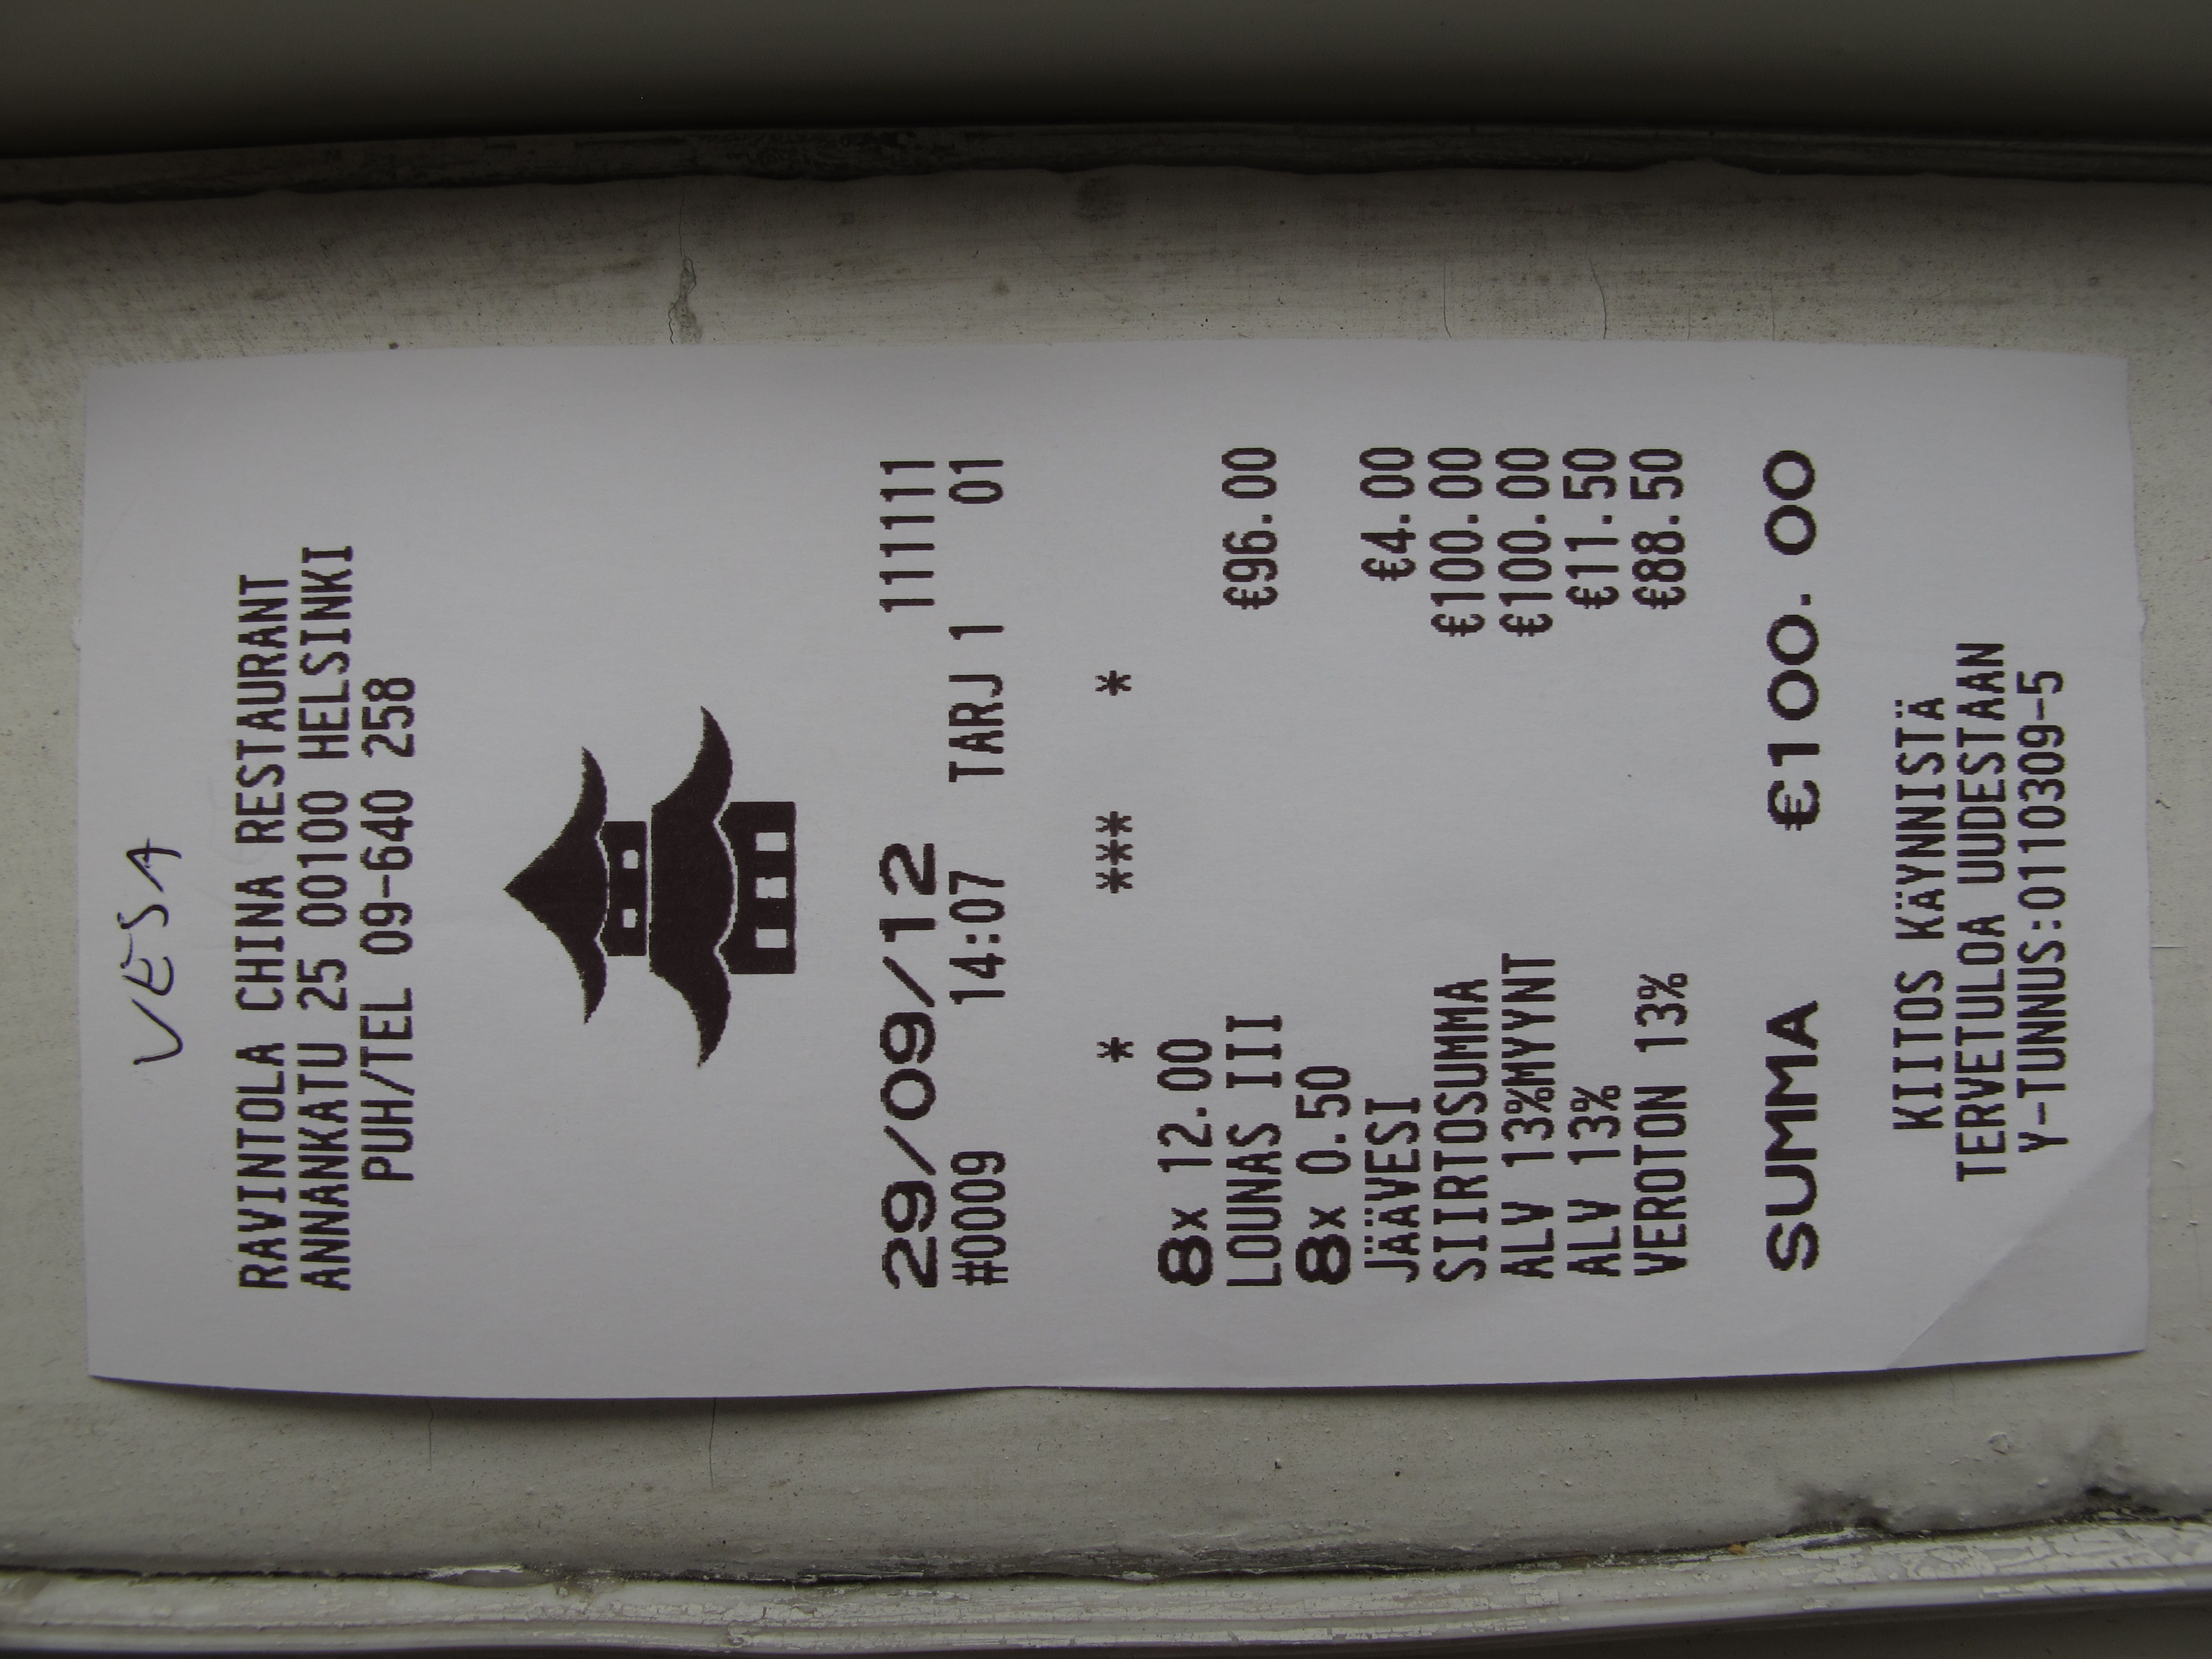
\includegraphics[width=80mm, angle=270]{pictures/alv-kuitti}
    \begin{vastaus}
         $13~\%$ sadasta eurosta on $13$ euroa, ei $11,50$ euroa, niin kuin kuitissa todetaan. Arvonlisävero
         lasketaan suhteessa verottomaan hintaan, ei lopulliseen myyntihintaan.
    \end{vastaus}
\end{tehtava}

\begin{tehtava}
    Laukun normaalihinta on $225$ euroa, ja se on $25$ prosentin alennuksessa.
    Mikä on alennettu hinta?
    \begin{vastaus}
        $168,75$ euroa
    \end{vastaus}
\end{tehtava}

\begin{tehtava}
    Jaakon kuukausipalkka on $1623,52$ euroa. Hän saa $1,3\,\%$ palkankorotuksen.
    Mikä on Jaakon kuukausipalkka korotuksen jälkeen?
    \begin{vastaus}
        $1644,63$ euroa
    \end{vastaus}
\end{tehtava}

\begin{tehtava}
    Kirjan myyntihinta, joka sisältää arvolisäveron, on $9\,\%$ suurempi kuin kirjan veroton hinta.
    Laske kirjan veroton hinta, kun myyntihinta on $27$ euroa.
    \begin{vastaus}
        Kirjan veroton hinta on $24,77$ euroa.
    \end{vastaus}
\end{tehtava}

\begin{tehtava}
    Sokerijuurikkaassa on $18~\%$ sokeria. Kuinka paljon sokerijuurikkaita tarvitaan valmistettaessa
    $8$ tonnia sokeriliuosta, jonka sokeripitoisuus on $4,5\,\%$?
    \begin{vastaus}
        $2$ tonnia
    \end{vastaus}
\end{tehtava}

\begin{tehtava}
    Perussuomalaisten kannatus oli vuoden 2007 eduskuntavaaleissa $4,1\,\%$ ja 
    vuoden 2011 eduskuntavaaleissa $19,1\,\%$. Kuinka monta prosenttiyksikköä 
    kannatus nousi? Kuinka monta prosenttia kannatus nousi?
    \begin{vastaus}
        Kannatus nousi $15$ prosenttiyksikköä, ja toisaalta $366$ prosenttia.
        Mediassa kannatusmuutokset ilmoitetaan yleensä prosenttiyksiköissä.
    \end{vastaus}
\end{tehtava}

\begin{tehtava}
    Askartelukaupassa on alennusviikot, ja kaikki tavarat myydään $60\,\%$:n 
    alennuksella. Viimeisenä päivänä kaikista hinnoista annetaan vielä 
    lisäalennus, joka lasketaan aiemmin alennetusta hinnasta. Minkä suuruinen 
    lisäalennus tulee antaa, jos lopullisen kokonaisalennuksen halutaan olevan $80\,\%$?
    \begin{vastaus}
        $50\,\%$
    \end{vastaus}
\end{tehtava}

\begin{tehtava}
    Hedelmissä on vettä aluksi $60\,\%$ niiden painosta. Kuinka monta prosenttia vedestä on haihdutettava, jotta hedelmissä tämän jälkeen olisi vain $20\,\%$ vettä?
    \begin{vastaus}
        $50\,\%$
    \end{vastaus}
\end{tehtava}


\begin{tehtava}
    Samulin pituus on $165$\,cm ja Joonaksen $173$\,cm.
    \begin{alakohdat}
        \alakohta{Kuinka monta prosenttia Samulin pituus on Joonaksen pituudesta?}
        \alakohta{Kuinka monta prosenttia Joonaksen pituus on Samulin pituudesta?}
        \alakohta{Kuinka monta prosenttia Samuli on lyhyempi kuin Joonas?}
        \alakohta{Kuinka monta prosenttia Joonas on pidempi kuin Samuli?}
    \end{alakohdat}
    \begin{vastaus}
        \begin{alakohdat}
            \alakohta{$95,4\,\%$}
            \alakohta{$104{,}8\,\%$}
            \alakohta{$4,62\,\%$}
            \alakohta{$4,85\,\%$}
        \end{alakohdat}
    \end{vastaus}
\end{tehtava}

\begin{tehtava}
    Vuonna 2012 yleinen arvonlisäveroprosentti Suomessa oli $23\,\%$ tuotteen
    verottomasta hinnasta. Tuotteen hinta koostuu sen verottomasta hinnasta 
    ja tuotteesta maksettavasta arvonlisäverosta. Kuinka monta 
    prosenttia arvonlisävero on tuotteen myyntihinnasta?
    \begin{vastaus}
        $18,7\,\%$
    \end{vastaus}
\end{tehtava}

\begin{tehtava}
    Kun matkalipun hintaa korotettiin $10,0\,\%$, matkustajien määrä väheni $10,0\,\%$.
    Kuinka monella prosentilla tällöin kasvoivat tai vähenivät liikennöitsijän 
    lipputulot?
    \begin{vastaus}
        Lipputulot vähenivät $1$~prosentilla.
    \end{vastaus}
\end{tehtava}


%Lisännyt Aleksi Sipola 10.11.2013
\begin{tehtava}
    (YO 1991K 5a) Luvun $\sqrt{r^2-a^2}$ likiarvona voidaan käyttää lukua $r-{\frac{1}{2}a^2}/r$. Laske tämän nojalla $\sqrt{3}$ likiarvo sopivia kokonaislukuja r ja a käyttäen. Kuinka monta prosenttia tämä likiarvo poikkeaa tarkasta arvosta?
    \begin{vastaus}
        Likiarvo on $1.75$ ja $\sqrt{3}=1.732...$. Likiarvo poikkeaa noin $1,04\,\%$.
    \end{vastaus}
\end{tehtava}

\begin{tehtava}
    Tuoreissa omenissa on vettä $80\,\%$ ja sokeria $4\,\%$. Kuinka monta prosenttia sokeria on samoissa omenissa, kun ne on kuivattu siten, että kosteusprosentti on $20$? [K2000, 4]
    \begin{vastaus}
        $16\,\%$
    \end{vastaus}
\end{tehtava}

\begin{tehtava}
    Matin ja Iidan duo saa julkisuutta, ja he alkavat myydä CD-levyään keikkojen yhteydessä $10$ euron
    kappalehinnalla. Jonkin ajan päästä he päättävät laskea CD-levyn hintaa $20$ prosenttia. Matti alkaa
    kuitenkin katua päätöstä, ja ehdottaa tämän alennetun hinnan korottamista $20$ prosentilla. Mikä olisi
    tämän toimenpiteen jälkeen CD:n uusi hinta? Montako prosenttia olisi korotuksen oltava, jotta oikeasti
    päästäisiin takaisin alkuperäiseen $10$ euron hintaan?
    \begin{vastaus}
        $25\,\%$
    \end{vastaus}
\end{tehtava}

\begin{tehtava}
    Jalkapalloilija Georgios Samaras teki ensimmäisellä kaudellaan Skotlannin valioliigassa (2007-08)
    $5$ maalia Celtic F.C.:n paidassa. Seuraavalla kaudella Samaras teki Celticille liigassa $15$ maalia.
    Kuinka monta prosenttia Samaraksen maalimäärä nousi?
    \begin{vastaus}
        $200\,\%$
    \end{vastaus}
\end{tehtava}

\begin{tehtava}
    Kaupungissa tuli jokaisen talonomistajan suorittaa kaupungin kassaan $5\,\%$ saadusta
    hyyrymäärästä (vuokrasta, ruotsin sanasta \textit{hyra}). Sittemmin määrättiin, että mainittu
    prosentti oli oleva 10. Monellako prosentilla täytyy talonomistajien korottaa hyyryjä
    saadakseen saman puhtaan säästön kuin ennen? [YO 1877, 4]
    \begin{vastaus}
        $5,6\,\%$
    \end{vastaus}
\end{tehtava}

\end{tehtavasivu}
